\begin{Exercise}[title=(*) Spectromètre de masse ]
	\begin{minipage}{.45\linewidth}
	Un spectromètre de masse permet de mesurer la masse des particules avec une telle précision qu'il peut servir à déterminer des compositions isotopique d'élément chimique. On s'intéresse ici au cas du Mercure.
	Une source émet des ions mercures $^{200}_{80} Hg^{2+}$ $^{202}_{80}Hg^{2+}$. ces ions passent dans le spectromètre de masse où ils ont accélérés puis séparer afins de mesurer leur rapport isotopique.\\
	\emph{Données numériques:} \\
	$d=1$ m ; $U= 1,00.10^4$ V; unité de masse atomique $1u=1,67.10^{27}$kg (masse d'un nucléon); $E_1=5,30.10^4$V/m; $B_1=0,383$T; $B_2=0,2$T; $F_3O_1=1.44$m $F_3O_2=$1.45m
	\end{minipage}\hspace{.05\linewidth}
	\begin{minipage}{0.45\textwidth}
		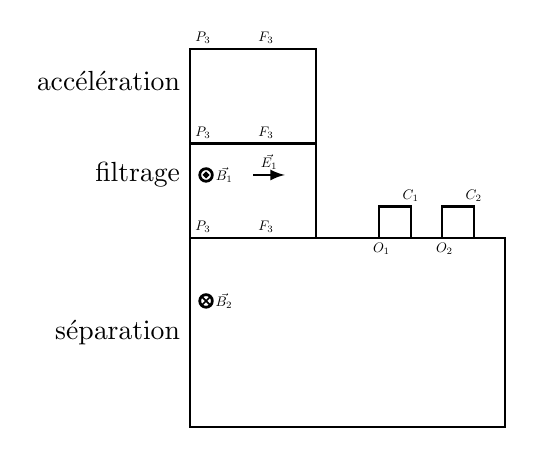
\begin{tikzpicture}[thick,scale=0.4, every node/.style={scale=0.5}]
	\draw (0,0) rectangle (10,6);
	\draw (6,6) rectangle ++(1,1) node[above]{$C_1$};
	
	\draw (6.5,6) node[below left]{$O_1$}
  node[color=white]{$\blacksquare$};
	\draw (8,6) rectangle ++(1,1)node[above]{$C_2$};
	\draw (8.5,6) node[below left]{$O_2$}
  node[color=white]{$\blacksquare$};
	\draw (0,6) node[above right]{$P_3$} -- ++(4,0) 
				node[midway,above right]{$F_3$} 
				node[midway,color=white]{$\blacksquare$};
	\draw (0,6)--(0,9) 
				node[above right]{$P_3$} -- ++(4,0) 
				node[midway,above right]{$F_3$} 
				node[midway,color=white]{$\blacksquare$} -- ++(0,-3);
	\draw (0,9)--(0,12) 
				node[above right]{$P_3$} -- ++(4,0) 
				node[midway,above right]{$F_3$} 
				node[midway,color=white]{$\blacksquare$} -- ++(0,-3);
	\filldraw[fill=white,line width=1pt](.5,4)circle(.2cm);
	\draw[line width=.6pt] (.5,4) node[right]{$~\vec{B_2}$}
	+(-135:.2cm) -- +(45:.2cm)
	+(-45:.2cm) -- +(135:.2cm);
	\filldraw[fill=white,line width=1pt](.5,8)circle(.2cm);
	\filldraw[fill=black,line width=1pt](.5,8)circle(.05cm) node[right]{$~\vec{B_1}$};
	\draw[>=latex,->] (2,8) -- (3,8) 		
						node[midway,above]{$\vec{E_1}$};
	\node[scale=2,left] at(0,3){séparation};
	\node[scale=2,left] at(0,8){filtrage};
	\node[scale=2,left] at(0,11){accélération};
\end{tikzpicture}
	\end{minipage}
		\Question Accélération des ions
		\subQuestion Préciser la plaque de potentiel le plus élevé, calculer numériquement la valeur de champ $E_0$.
		\subQuestion Établir l'expression littérale de la vitesse $v_0$ des ions sur la plaque $P_2$.
		\subQuestion Calculer numériquement $v_01$ et $v_02$. les vitesses respectives des deux isotopes du mercure à lerur arrivé en $F_2$.
		\emph{Étant donnée que l'hypothèse de vitesse nulle en $F_1$ est difficile à réalisé en pratique,
                   il est nécessaire de filtrer en vitesse pour améliore les performances  de l'appareil}.
		\Question Filtre en vitesse.\\
		Les ions traverse la plaque $P_2$ par la fente $F_2$avec un vitesse perpendiculaire à $P_2$ Ils entrent dans l'espace séparent $P_2$ et $P_3$ où règne:
		-- un champ $\vec{E_1}$ parallèle à $P_2$ et dans le plan du schéma. \\
		-- un champ $\vec{B_1}$ uniforme et perpendiculaire au plan du schéma.
		\subQuestion Sous quelles conditions les ions peuvent-ils avoir une trajectoire rectiligne les amenant jusqu'en $F_3$?
		\subQuestion Calculer numériquement cette vitesse et en déduire quel isotope du mercure arrive en $F_3$ avec ces réglages.
		\Question Séparation des ions
		Après $F_3$ les ions pénètrent dans une région où ne règne qu'un champ magnétique $\vec{B_2}$ normal au plan du schéma. ils sont déviés vers les collecteurs $C_1$ et $C_2$.
		\subQuestion Montrer que le mouvement des ions dans cette région est uniforme.
		\subQuestion Sachant que la trajectoire des ions est circulaire, déterminer les rayons des  demis cercles décris par les deux isotopes.
		\subQuestion Associer chaque collecteur à l'isotope correspondant.
		\subQuestion La distance $\delta$ qui sépare les points $O_1$ et $O_2$ parait-elle suffisante pour pouvoir installer des détecteurs de particules?
		\subQuestion les quantités d'électricité reçu en une minute par les collecteurs sont $Q_1=1,20.10^{-7}$C et $Q_2=3,5.10^{-8}$C. Déterminer la composition isotopique du mercure. en déduire sa masse atomique.
\end{Exercise}
\begin{Answer}
		\Question
		\subQuestion les ions sont positifs ,pour accélérer on veux $\vec{E}$ dans le sens de l'accélération, le champs descend les potentiels donc les charges sont en $P_1$. $\vec{E_0} = \frac{U}{d}\vec{u_x}$ et \gdr{E_0}{1e4}{\V\per\m}
		\subQuestion TEC : $v_0=\sqrt{\frac{2qU}{m}}$
		\subQuestion \gdr{v_{01}}{1,384e5}{\v} et \gdr{v_{02}}{1.377e5}{\v}
		\Question on veut $\vec{f_B}$ opposée à $\vec{f_E}$ donc \gdr{v_0 = E_1/B_1}{1.384e5}{\v}.  c'est l'isotope 200 qui parvient en $F_3$ l'isotope 202 est lui \textit{dévié vers la droite}
		\Question TEC  : $m\frac{v_0^2}{R}=qv_0B_2$ donc $R=\frac{mv_0}{qB_2}$ on  a \gdr{R_1}{0.722}{m} \gdr{R_2}{0,726}{m}.$C_1$ reçoit les isotopes 200, $C_2$ les isotopes 202.
\end{Answer}
